%!TEX root = ../index.tex

%
% Implementation
%

\section{Implementation}

Every code artifact was developed following the Unix philosophy, every module attempts to do at most one thing and one thing well, creating small, maintainable and powerful abstractions.

\subsection{Browser module}

The browser module is the agent that sits inside our browser nodes, implementing all the communication protocols designed for the browserCloud.js platform and exposing a developer API to send and receive messages.

Essentially it is broken down into 4 components:

\begin{itemize}
    \item channel manager - responsible to leverage the websockets connection with the signalling server and abstracts the necessary work to open new RTCPeerConnections with other peers.
    \item finger table manager - where the information about a specific peer finger table lives.
    \item router - the routing logic to deliver the messages on the most efficient way. It uses the finger table manager to understand what is the most efficient way to rout messages.
    \item interface - developer exposed interface.
\end{itemize}

\subsection{Signalling server}

The Signalling Server offers a HTTP and Web Sockets API and serves as a rendezvous point for SDP data exchange between browsers so they can establish a RTCPeerConnection. 

\subsection{Testing framework - piri-piri}

The testing framework implementation, which we named "piri-piri", encapsulates the necessary logic described on section 3.5.

\subsection{Visualize the network state}

Using D3JS\footnote{http://d3js.org}, we have developed an application that grabs the state of the browserCloud.js network and shows a live graphical representation, as seen on Figure~\ref{fig:visualizer}, where each node is represented by a dot and its ID and the arcs being the connections established between the nodes in the network. 

\begin{figure}[h!]
  \centering
  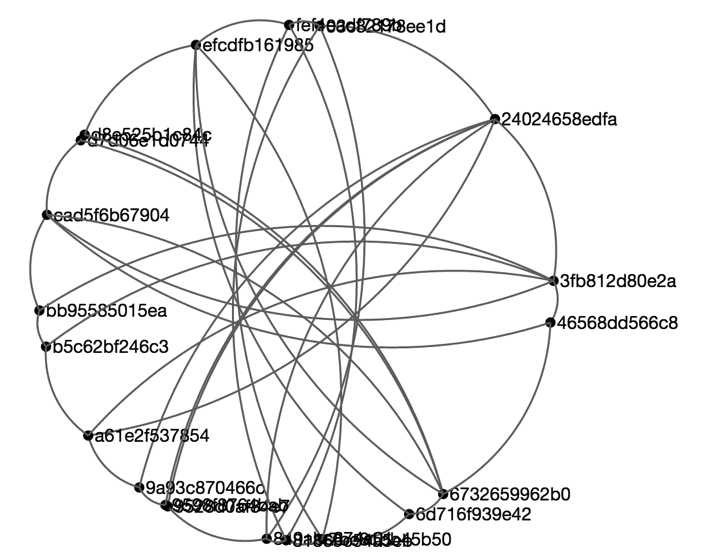
\includegraphics[width=0.35\textwidth]{figs/visualizer}
  \caption{Visualization of a browserCloud.js network}
  \label{fig:visualizer}
\end{figure}

\subsection{Ray Tracing module}

To perform the parallel CPU bound tests, we have developed a module that works in Node.js and in the browser to perform Ray Tracing Tasks.
